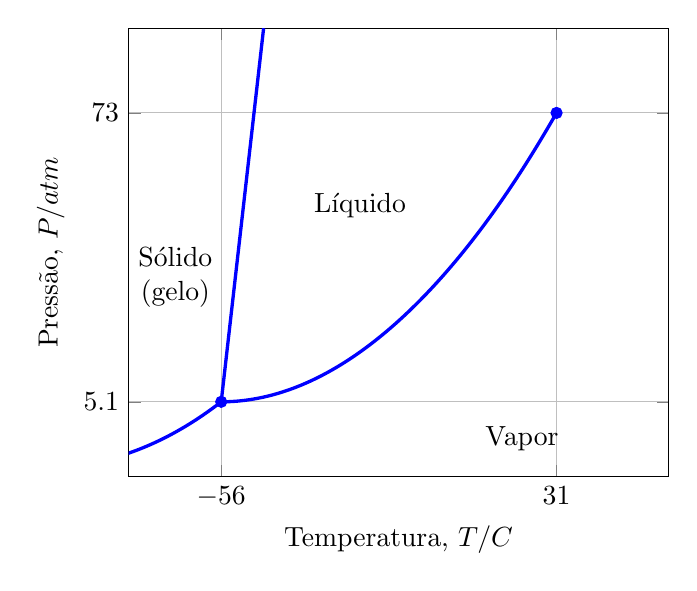
\begin{tikzpicture}
\begin{axis}
    [
        grid = major,
        ylabel = {Pressão, $P/\unit{atm}$},
        xlabel = {Temperatura, $T/\unit{\degree C}$},
        ymin=0, ymax=90,
        xmin=-80
        , xmax=60,
        ytick = { 15, 73 },
        yticklabels = { \num{5.1}, \num{73} },
        xtick = { -56, 31 },
    ]       
    \draw [draw=blue, very thick]
        (axis cs: -100, 2) parabola 
        (axis cs: -56, 15);
    \draw [draw=blue, very thick]
        (axis cs: -56, 15) parabola 
        (axis cs: 31, 73);
    \draw [draw=blue, very thick]
        (axis cs: -56, 15) -- 
        (axis cs: -45, 90);
    
    \addplot [ mark=*, color=blue, only marks ] coordinates
        { 
            (-56, 15)
            (31, 73)
        };

    \node [anchor = west, align = center] at (axis cs:-80, 40) 
        { Sólido \\ (gelo) };
    \node [anchor = south] at (axis cs:-20, 50) 
        { Líquido };
    \node [anchor = west] at (axis cs:10, 7.5) 
        { Vapor };
        
\end{axis}
\end{tikzpicture}
